% Options for packages loaded elsewhere
\PassOptionsToPackage{unicode}{hyperref}
\PassOptionsToPackage{hyphens}{url}
\PassOptionsToPackage{dvipsnames,svgnames,x11names}{xcolor}
%
\documentclass[
  letterpaper,
  DIV=11,
  numbers=noendperiod]{scrreprt}

\usepackage{amsmath,amssymb}
\usepackage{iftex}
\ifPDFTeX
  \usepackage[T1]{fontenc}
  \usepackage[utf8]{inputenc}
  \usepackage{textcomp} % provide euro and other symbols
\else % if luatex or xetex
  \usepackage{unicode-math}
  \defaultfontfeatures{Scale=MatchLowercase}
  \defaultfontfeatures[\rmfamily]{Ligatures=TeX,Scale=1}
\fi
\usepackage{lmodern}
\ifPDFTeX\else  
    % xetex/luatex font selection
\fi
% Use upquote if available, for straight quotes in verbatim environments
\IfFileExists{upquote.sty}{\usepackage{upquote}}{}
\IfFileExists{microtype.sty}{% use microtype if available
  \usepackage[]{microtype}
  \UseMicrotypeSet[protrusion]{basicmath} % disable protrusion for tt fonts
}{}
\makeatletter
\@ifundefined{KOMAClassName}{% if non-KOMA class
  \IfFileExists{parskip.sty}{%
    \usepackage{parskip}
  }{% else
    \setlength{\parindent}{0pt}
    \setlength{\parskip}{6pt plus 2pt minus 1pt}}
}{% if KOMA class
  \KOMAoptions{parskip=half}}
\makeatother
\usepackage{xcolor}
\setlength{\emergencystretch}{3em} % prevent overfull lines
\setcounter{secnumdepth}{5}
% Make \paragraph and \subparagraph free-standing
\makeatletter
\ifx\paragraph\undefined\else
  \let\oldparagraph\paragraph
  \renewcommand{\paragraph}{
    \@ifstar
      \xxxParagraphStar
      \xxxParagraphNoStar
  }
  \newcommand{\xxxParagraphStar}[1]{\oldparagraph*{#1}\mbox{}}
  \newcommand{\xxxParagraphNoStar}[1]{\oldparagraph{#1}\mbox{}}
\fi
\ifx\subparagraph\undefined\else
  \let\oldsubparagraph\subparagraph
  \renewcommand{\subparagraph}{
    \@ifstar
      \xxxSubParagraphStar
      \xxxSubParagraphNoStar
  }
  \newcommand{\xxxSubParagraphStar}[1]{\oldsubparagraph*{#1}\mbox{}}
  \newcommand{\xxxSubParagraphNoStar}[1]{\oldsubparagraph{#1}\mbox{}}
\fi
\makeatother

\usepackage{color}
\usepackage{fancyvrb}
\newcommand{\VerbBar}{|}
\newcommand{\VERB}{\Verb[commandchars=\\\{\}]}
\DefineVerbatimEnvironment{Highlighting}{Verbatim}{commandchars=\\\{\}}
% Add ',fontsize=\small' for more characters per line
\usepackage{framed}
\definecolor{shadecolor}{RGB}{241,243,245}
\newenvironment{Shaded}{\begin{snugshade}}{\end{snugshade}}
\newcommand{\AlertTok}[1]{\textcolor[rgb]{0.68,0.00,0.00}{#1}}
\newcommand{\AnnotationTok}[1]{\textcolor[rgb]{0.37,0.37,0.37}{#1}}
\newcommand{\AttributeTok}[1]{\textcolor[rgb]{0.40,0.45,0.13}{#1}}
\newcommand{\BaseNTok}[1]{\textcolor[rgb]{0.68,0.00,0.00}{#1}}
\newcommand{\BuiltInTok}[1]{\textcolor[rgb]{0.00,0.23,0.31}{#1}}
\newcommand{\CharTok}[1]{\textcolor[rgb]{0.13,0.47,0.30}{#1}}
\newcommand{\CommentTok}[1]{\textcolor[rgb]{0.37,0.37,0.37}{#1}}
\newcommand{\CommentVarTok}[1]{\textcolor[rgb]{0.37,0.37,0.37}{\textit{#1}}}
\newcommand{\ConstantTok}[1]{\textcolor[rgb]{0.56,0.35,0.01}{#1}}
\newcommand{\ControlFlowTok}[1]{\textcolor[rgb]{0.00,0.23,0.31}{\textbf{#1}}}
\newcommand{\DataTypeTok}[1]{\textcolor[rgb]{0.68,0.00,0.00}{#1}}
\newcommand{\DecValTok}[1]{\textcolor[rgb]{0.68,0.00,0.00}{#1}}
\newcommand{\DocumentationTok}[1]{\textcolor[rgb]{0.37,0.37,0.37}{\textit{#1}}}
\newcommand{\ErrorTok}[1]{\textcolor[rgb]{0.68,0.00,0.00}{#1}}
\newcommand{\ExtensionTok}[1]{\textcolor[rgb]{0.00,0.23,0.31}{#1}}
\newcommand{\FloatTok}[1]{\textcolor[rgb]{0.68,0.00,0.00}{#1}}
\newcommand{\FunctionTok}[1]{\textcolor[rgb]{0.28,0.35,0.67}{#1}}
\newcommand{\ImportTok}[1]{\textcolor[rgb]{0.00,0.46,0.62}{#1}}
\newcommand{\InformationTok}[1]{\textcolor[rgb]{0.37,0.37,0.37}{#1}}
\newcommand{\KeywordTok}[1]{\textcolor[rgb]{0.00,0.23,0.31}{\textbf{#1}}}
\newcommand{\NormalTok}[1]{\textcolor[rgb]{0.00,0.23,0.31}{#1}}
\newcommand{\OperatorTok}[1]{\textcolor[rgb]{0.37,0.37,0.37}{#1}}
\newcommand{\OtherTok}[1]{\textcolor[rgb]{0.00,0.23,0.31}{#1}}
\newcommand{\PreprocessorTok}[1]{\textcolor[rgb]{0.68,0.00,0.00}{#1}}
\newcommand{\RegionMarkerTok}[1]{\textcolor[rgb]{0.00,0.23,0.31}{#1}}
\newcommand{\SpecialCharTok}[1]{\textcolor[rgb]{0.37,0.37,0.37}{#1}}
\newcommand{\SpecialStringTok}[1]{\textcolor[rgb]{0.13,0.47,0.30}{#1}}
\newcommand{\StringTok}[1]{\textcolor[rgb]{0.13,0.47,0.30}{#1}}
\newcommand{\VariableTok}[1]{\textcolor[rgb]{0.07,0.07,0.07}{#1}}
\newcommand{\VerbatimStringTok}[1]{\textcolor[rgb]{0.13,0.47,0.30}{#1}}
\newcommand{\WarningTok}[1]{\textcolor[rgb]{0.37,0.37,0.37}{\textit{#1}}}

\providecommand{\tightlist}{%
  \setlength{\itemsep}{0pt}\setlength{\parskip}{0pt}}\usepackage{longtable,booktabs,array}
\usepackage{calc} % for calculating minipage widths
% Correct order of tables after \paragraph or \subparagraph
\usepackage{etoolbox}
\makeatletter
\patchcmd\longtable{\par}{\if@noskipsec\mbox{}\fi\par}{}{}
\makeatother
% Allow footnotes in longtable head/foot
\IfFileExists{footnotehyper.sty}{\usepackage{footnotehyper}}{\usepackage{footnote}}
\makesavenoteenv{longtable}
\usepackage{graphicx}
\makeatletter
\def\maxwidth{\ifdim\Gin@nat@width>\linewidth\linewidth\else\Gin@nat@width\fi}
\def\maxheight{\ifdim\Gin@nat@height>\textheight\textheight\else\Gin@nat@height\fi}
\makeatother
% Scale images if necessary, so that they will not overflow the page
% margins by default, and it is still possible to overwrite the defaults
% using explicit options in \includegraphics[width, height, ...]{}
\setkeys{Gin}{width=\maxwidth,height=\maxheight,keepaspectratio}
% Set default figure placement to htbp
\makeatletter
\def\fps@figure{htbp}
\makeatother
% definitions for citeproc citations
\NewDocumentCommand\citeproctext{}{}
\NewDocumentCommand\citeproc{mm}{%
  \begingroup\def\citeproctext{#2}\cite{#1}\endgroup}
\makeatletter
 % allow citations to break across lines
 \let\@cite@ofmt\@firstofone
 % avoid brackets around text for \cite:
 \def\@biblabel#1{}
 \def\@cite#1#2{{#1\if@tempswa , #2\fi}}
\makeatother
\newlength{\cslhangindent}
\setlength{\cslhangindent}{1.5em}
\newlength{\csllabelwidth}
\setlength{\csllabelwidth}{3em}
\newenvironment{CSLReferences}[2] % #1 hanging-indent, #2 entry-spacing
 {\begin{list}{}{%
  \setlength{\itemindent}{0pt}
  \setlength{\leftmargin}{0pt}
  \setlength{\parsep}{0pt}
  % turn on hanging indent if param 1 is 1
  \ifodd #1
   \setlength{\leftmargin}{\cslhangindent}
   \setlength{\itemindent}{-1\cslhangindent}
  \fi
  % set entry spacing
  \setlength{\itemsep}{#2\baselineskip}}}
 {\end{list}}
\usepackage{calc}
\newcommand{\CSLBlock}[1]{\hfill\break\parbox[t]{\linewidth}{\strut\ignorespaces#1\strut}}
\newcommand{\CSLLeftMargin}[1]{\parbox[t]{\csllabelwidth}{\strut#1\strut}}
\newcommand{\CSLRightInline}[1]{\parbox[t]{\linewidth - \csllabelwidth}{\strut#1\strut}}
\newcommand{\CSLIndent}[1]{\hspace{\cslhangindent}#1}

\KOMAoption{captions}{tableheading}
\makeatletter
\@ifpackageloaded{tcolorbox}{}{\usepackage[skins,breakable]{tcolorbox}}
\@ifpackageloaded{fontawesome5}{}{\usepackage{fontawesome5}}
\definecolor{quarto-callout-color}{HTML}{909090}
\definecolor{quarto-callout-note-color}{HTML}{0758E5}
\definecolor{quarto-callout-important-color}{HTML}{CC1914}
\definecolor{quarto-callout-warning-color}{HTML}{EB9113}
\definecolor{quarto-callout-tip-color}{HTML}{00A047}
\definecolor{quarto-callout-caution-color}{HTML}{FC5300}
\definecolor{quarto-callout-color-frame}{HTML}{acacac}
\definecolor{quarto-callout-note-color-frame}{HTML}{4582ec}
\definecolor{quarto-callout-important-color-frame}{HTML}{d9534f}
\definecolor{quarto-callout-warning-color-frame}{HTML}{f0ad4e}
\definecolor{quarto-callout-tip-color-frame}{HTML}{02b875}
\definecolor{quarto-callout-caution-color-frame}{HTML}{fd7e14}
\makeatother
\makeatletter
\@ifpackageloaded{bookmark}{}{\usepackage{bookmark}}
\makeatother
\makeatletter
\@ifpackageloaded{caption}{}{\usepackage{caption}}
\AtBeginDocument{%
\ifdefined\contentsname
  \renewcommand*\contentsname{Table of contents}
\else
  \newcommand\contentsname{Table of contents}
\fi
\ifdefined\listfigurename
  \renewcommand*\listfigurename{List of Figures}
\else
  \newcommand\listfigurename{List of Figures}
\fi
\ifdefined\listtablename
  \renewcommand*\listtablename{List of Tables}
\else
  \newcommand\listtablename{List of Tables}
\fi
\ifdefined\figurename
  \renewcommand*\figurename{Figure}
\else
  \newcommand\figurename{Figure}
\fi
\ifdefined\tablename
  \renewcommand*\tablename{Table}
\else
  \newcommand\tablename{Table}
\fi
}
\@ifpackageloaded{float}{}{\usepackage{float}}
\floatstyle{ruled}
\@ifundefined{c@chapter}{\newfloat{codelisting}{h}{lop}}{\newfloat{codelisting}{h}{lop}[chapter]}
\floatname{codelisting}{Listing}
\newcommand*\listoflistings{\listof{codelisting}{List of Listings}}
\makeatother
\makeatletter
\makeatother
\makeatletter
\@ifpackageloaded{caption}{}{\usepackage{caption}}
\@ifpackageloaded{subcaption}{}{\usepackage{subcaption}}
\makeatother

\ifLuaTeX
  \usepackage{selnolig}  % disable illegal ligatures
\fi
\usepackage{bookmark}

\IfFileExists{xurl.sty}{\usepackage{xurl}}{} % add URL line breaks if available
\urlstyle{same} % disable monospaced font for URLs
\hypersetup{
  pdftitle={Data Management},
  pdfauthor={Moses Otieno},
  colorlinks=true,
  linkcolor={blue},
  filecolor={Maroon},
  citecolor={Blue},
  urlcolor={Blue},
  pdfcreator={LaTeX via pandoc}}


\title{Data Management}
\author{Moses Otieno}
\date{2024-08-10}

\begin{document}
\maketitle

\renewcommand*\contentsname{Table of contents}
{
\hypersetup{linkcolor=}
\setcounter{tocdepth}{2}
\tableofcontents
}

\bookmarksetup{startatroot}

\chapter*{Preface}\label{preface}
\addcontentsline{toc}{chapter}{Preface}

\markboth{Preface}{Preface}

\section*{What is this tutorial
about?}\label{what-is-this-tutorial-about}
\addcontentsline{toc}{section}{What is this tutorial about?}

\markright{What is this tutorial about?}

This tutorial provides a comprehensive guide to building a data
management pipeline using various programming languages and tools. It
aims at equiping you with the knowledge and skills necessary to
efficiently collect, manage, and analyze data, particularly in the
context of survey data.

You will learn how to leverage \textbf{R} for data manipulation and
reporting, utilize \textbf{Python} for scripting and automation, and
manage databases with \textbf{MySQL}. Additionally, the tutorial will
introduce you to \textbf{Batch scripting} for task automation in Windows
environments.

A key focus will be on \textbf{Survey Solutions}, a robust platform for
data collection, where you will gain familiarity with its API for
downloading and managing survey data. By working with the \texttt{ssaw}
Python package, you will learn how to integrate these tools to create a
seamless data management pipeline.

Overall, this tutorial is designed for individuals who have a basic
understanding of the prerequisites and are looking to enhance their
skills in data management and analysis through practical, hands-on
experience.

\section*{Prerequisites}\label{prerequisites}
\addcontentsline{toc}{section}{Prerequisites}

\markright{Prerequisites}

Before starting this tutorial, ensure you have a basic understanding of
the following:

\textbf{Survey Solutions}

\begin{itemize}
\tightlist
\item
  Basic understanding of the Survey Solutions platform.
\item
  Familiarity with its API for downloading and managing survey data.
\item
  Ability to work with the \texttt{ssaw} Python package for Survey
  Solutions integration.
\end{itemize}

\textbf{Python}

\begin{itemize}
\item
  Experience with scripting and automation.
\item
  Knowledge of using libraries like \texttt{pandas} for data
  manipulation.
\item
  Ability to integrate Python scripts with APIs.
\end{itemize}

\textbf{R}

\begin{itemize}
\item
  Familiarity with data manipulation and reporting.
\item
  Comfortable working with data frames and R scripts.
\item
  Ability to use packages for data analysis.
\end{itemize}

\textbf{MySQL}

\begin{itemize}
\item
  Understanding of database management and querying.
\item
  Ability to create databases and write SQL queries.
\item
  Comfortable managing data in MySQL environments.
\end{itemize}

\textbf{Batch Scripting}:

\begin{itemize}
\item
  Familiarity with automating tasks in Windows.
\item
  Ability to write and run batch files for task automation.
\end{itemize}

\begin{tcolorbox}[enhanced jigsaw, colframe=quarto-callout-note-color-frame, rightrule=.15mm, title=\textcolor{quarto-callout-note-color}{\faInfo}\hspace{0.5em}{Note}, toprule=.15mm, coltitle=black, left=2mm, opacitybacktitle=0.6, colback=white, bottomrule=.15mm, leftrule=.75mm, opacityback=0, breakable, titlerule=0mm, bottomtitle=1mm, colbacktitle=quarto-callout-note-color!10!white, toptitle=1mm, arc=.35mm]

While proficiency is not required in any of these areas, a good level of
familiarity will be beneficial for following the tutorial.

\end{tcolorbox}

\bookmarksetup{startatroot}

\chapter{Introduction}\label{introduction}

This tutorial is about automating data management and report writing.
The growing need for timely, accurate, and efficient data processing has
made automation not just a luxury but a necessity in modern data
management practices. This tutorial will take you on a step-by-step
journey to streamline your data management processes by leveraging four
powerful tools: Batch scripting, Python, SQL, and R.

Survey Solutions, a widely-used survey data collection platform, offers
rich capabilities for collecting complex datasets. However, the true
power lies in how quickly and effectively you can automate the
retrieval, cleaning, and analysis of this data. This tutorial aims to
bridge that gap. Whether you're managing data for health research,
social impact projects, or other sectors, automating the extraction and
transformation of data will save hours of manual work and reduce the
risk of human error.

In this tutorial, we will walk you through creating a robust data
management pipeline, starting with Python to download data from the
Survey Solutions via API. We will then transition to R to perform
in-depth data management and generate dynamic reports. After the reports
have been generated will get back to Python then share the reports with
the stake-holders. We will then use SQL to track the progress of report
sharing. Batch scripts will be used in automating all these processes.
By the end of this guide, you will have a seamless workflow that not
only automates your data processes but also enhances their accuracy and
scalability.

\bookmarksetup{startatroot}

\chapter{Data Download}\label{data-download}

\section{Introduction}\label{introduction-1}

In the ever-evolving landscape of data collection,
\href{https://mysurvey.solutions/en/}{Survey Solutions} stands out as a
powerful and versatile tool designed to streamline the process.
Developed by the World Bank, this innovative platform enables
researchers and organizations to gather high-quality data efficiently
and effectively. With its user-friendly interface and robust features,
Survey Solutions empowers field staff to conduct surveys, manage complex
questionnaires, and ensure data integrity in real-time.

One of the standout capabilities of Survey Solutions is its robust API,
which allows for seamless integration with other systems and
applications. This feature enables users to automate data collection
processes, enhance data management, and facilitate real-time data
access, making it easier to incorporate Survey Solutions into existing
workflows.

By harnessing the capabilities of Survey Solutions, users can customize
surveys to meet specific research needs, collect data through mobile
devices, and utilize advanced tools for monitoring and data analysis.
This flexibility not only enhances the quality of data collected but
also accelerates decision-making processes in various sectors, including
healthcare, education, and social research.

Whether you're a seasoned researcher or a novice data collector, Survey
Solutions provides the resources and support necessary to transform data
collection into a seamless and impactful experience. Embrace the future
of data gathering with Survey Solutions---where precision meets
efficiency.

\section{Survey Solution Accounts}\label{survey-solution-accounts}

In Survey Solutions, there are \textbf{six} main types of user accounts,
each with different roles and responsibilities. Here's a breakdown:

\begin{enumerate}
\def\labelenumi{\arabic{enumi}.}
\tightlist
\item
  \textbf{Administrator}:
\end{enumerate}

\begin{itemize}
\item
  \textbf{Role}: Manages the technical aspects of the Survey Solutions
  server.
\item
  \textbf{Responsibilities}:

  \begin{itemize}
  \item
    Set up and configure the Survey Solutions server.
  \item
    Manage server performance, updates, and backups.
  \item
    Handle user management (creation and deletion of accounts).
  \item
    Ensure security, including password management and system access.
  \item
    Monitor server health and log files.
  \end{itemize}
\end{itemize}

\begin{enumerate}
\def\labelenumi{\arabic{enumi}.}
\setcounter{enumi}{1}
\tightlist
\item
  \textbf{Headquarters (HQ)}:
\end{enumerate}

\begin{itemize}
\item
  \textbf{Role}: Manages the entire survey process, including
  questionnaire management, assignments, and overall data flow.
\item
  \textbf{Responsibilities}:

  \begin{itemize}
  \item
    Create and manage survey assignments.
  \item
    Monitor survey progress and interview status.
  \item
    Access all collected data.
  \item
    Administer users and roles.
  \item
    Handle questionnaire uploads and server management.
  \end{itemize}
\end{itemize}

\begin{enumerate}
\def\labelenumi{\arabic{enumi}.}
\setcounter{enumi}{2}
\tightlist
\item
  \textbf{Supervisor}:
\end{enumerate}

\begin{itemize}
\item
  \textbf{Role}: Oversees fieldwork operations, manages interviewers,
  and reviews their work.
\item
  \textbf{Responsibilities}:

  \begin{itemize}
  \item
    Review completed interviews submitted by interviewers.
  \item
    Approve or reject interviews.
  \item
    Manage interviewers and assignments within their team.
  \item
    Monitor the status of interviews and progress.
  \end{itemize}
\end{itemize}

\begin{enumerate}
\def\labelenumi{\arabic{enumi}.}
\setcounter{enumi}{3}
\tightlist
\item
  \textbf{Interviewer}:
\end{enumerate}

\begin{itemize}
\item
  \textbf{Role}: Conducts interviews and collects data in the field
  using a tablet or computer.
\item
  \textbf{Responsibilities}:

  \begin{itemize}
  \item
    Conduct face-to-face interviews with respondents.
  \item
    Upload collected data to the server for review.
  \item
    Communicate with supervisors on any issues related to interviews.
  \end{itemize}
\end{itemize}

\begin{enumerate}
\def\labelenumi{\arabic{enumi}.}
\setcounter{enumi}{4}
\tightlist
\item
  \textbf{Observer}:
\end{enumerate}

\begin{itemize}
\item
  \textbf{Role}: Has read-only access to monitor the progress of the
  survey without the ability to make changes.
\item
  \textbf{Responsibilities}:

  \begin{itemize}
  \item
    View interviews and their status.
  \item
    Generate reports and monitor survey performance.
  \item
    Cannot edit or approve interviews.
  \end{itemize}
\end{itemize}

\begin{enumerate}
\def\labelenumi{\arabic{enumi}.}
\setcounter{enumi}{5}
\tightlist
\item
  \textbf{API User}:
\end{enumerate}

\begin{itemize}
\item
  \textbf{Role}: Provides programmatic access to Survey Solutions
  through its API for automation and integration purposes.
\item
  \textbf{Responsibilities}:

  \begin{itemize}
  \item
    Fetch survey data via the API for external analysis.
  \item
    Automate the survey workflow by integrating with other systems
    (e.g., data processing or visualization tools).
  \item
    Create assignments, retrieve reports, and manage users
    programmatically.
  \end{itemize}
\end{itemize}

Of great importance for data management workflow is the API User. You
need to talk to the Administrator, who most of the times is either
system administrator or programmer, who set up and configured the Survey
Solutions server to create for you an API user.

\section{Survey Solution API}\label{survey-solution-api}

Survey Solutions includes a powerful and flexible
\href{https://docs.mysurvey.solutions/headquarters/api/survey-solutions-api/}{API}
which allows automating some tasks and allows our~users to build larger
systems, which may compliment Survey Solutions to achieve larger goals.~

Some examples of use could be:

\begin{itemize}
\item
  schedule periodic export of collected data
\item
  an external dashboard or monitoring and reporting system, which
  updates some indicators every night and publishes them to a website,
  or
\item
  an external checking and validation system which verifies collected
  data against some external sources of information and rejects
  automatically the incorrect interviews, or
\item
  an integrated system, which utilizes Survey Solutions for data
  collections tasks and a statistical package for continuous analysis,
\item
  facility management, inventory and price monitoring systems, etc, etc.
\end{itemize}

For the purposes of this tutorial, our focus will be on the first use
case.

\subsection{API Clients}\label{api-clients}

There are a number of API clients for Survey Solutions. They are listed
below.

\begin{longtable}[]{@{}
  >{\raggedright\arraybackslash}p{(\columnwidth - 6\tabcolsep) * \real{0.2676}}
  >{\raggedright\arraybackslash}p{(\columnwidth - 6\tabcolsep) * \real{0.2394}}
  >{\raggedright\arraybackslash}p{(\columnwidth - 6\tabcolsep) * \real{0.3239}}
  >{\raggedright\arraybackslash}p{(\columnwidth - 6\tabcolsep) * \real{0.1690}}@{}}
\toprule\noalign{}
\begin{minipage}[b]{\linewidth}\raggedright
API Clients
\end{minipage} & \begin{minipage}[b]{\linewidth}\raggedright
Maintainer
\end{minipage} & \begin{minipage}[b]{\linewidth}\raggedright
Specific Name
\end{minipage} & \begin{minipage}[b]{\linewidth}\raggedright
Language
\end{minipage} \\
\midrule\noalign{}
\endhead
\bottomrule\noalign{}
\endlastfoot
.NET package & Andrii Kozhyn & SurveySolutionsClient & C\# \\
PowerShell module & Zurab Sajaia & SSAW & Powershell \\
Python package & Zurab Sajaia & ssaw & Python \\
R package & Michael Wild & SurveySolutionsAPI & R \\
R package & Arthur Shaw & susoapi & R \\
R package & Lena Nguyen & SuSoAPI & R \\
Stata package & Sergiy Radyakin & susoapi & Stata \\
\end{longtable}

For more details about each of the clients you check
\href{https://docs.mysurvey.solutions/headquarters/api/survey-solutions-api/}{here}.

\section{Python Package}\label{python-package}

I use
\href{https://chatgpt.com/c/6704f64e-03fc-8012-9fcd-e574129e9878}{ssaw}
Python package as a Survey Solutions API wrapper. It is easy to use and
very flexible. We'll focus on key data management procedures, but full
details are in the
\href{https://chatgpt.com/c/6704f64e-03fc-8012-9fcd-e574129e9878}{online
documentation}.

\subsection{Installation}\label{installation}

To install ssaw, simply run this command in your terminal:

\begin{Shaded}
\begin{Highlighting}[]

\NormalTok{pip install ssaw}
\end{Highlighting}
\end{Shaded}

\subsection{Modules}\label{modules}

I use the following modules in data management pipeline especially when
working with Survey Solutions:

\begin{Shaded}
\begin{Highlighting}[]
\ImportTok{import}\NormalTok{ requests}
\ImportTok{from}\NormalTok{ ssaw }\ImportTok{import}\NormalTok{ Client, ExportApi, QuestionnairesApi, models}
\ImportTok{from}\NormalTok{ time }\ImportTok{import}\NormalTok{ sleep}
\ImportTok{import}\NormalTok{ configparser}
\ImportTok{import}\NormalTok{ os}
\end{Highlighting}
\end{Shaded}

\subsection{Connect to server}\label{connect-to-server}

To communicate with Survey Solutions server, you first need to
instantiate a client. You remember the API user you created or was
created for you? It is necessary at this point. To connect to Survey
Solution you need four pieces of information i.e.

\begin{itemize}
\item
  URL for the server
\item
  API username
\item
  API password
\item
  Name of the work space
\end{itemize}

\begin{description}
\item[\textbf{Parameters}]
\begin{itemize}
\item[]
\item
  \textbf{url} (\textbf{\texttt{str}}) -- URL of the headquarters app
\item
  \textbf{api\_user}
  (\textbf{\texttt{Optional}}{[}\textbf{\texttt{str}}{]}) -- API user
  name
\item
  \textbf{api\_password}
  (\textbf{\texttt{Optional}}{[}\textbf{\texttt{str}}{]}) -- API user
  password
\item
  \textbf{token} (\textbf{\texttt{Optional}}{[}\textbf{\texttt{str}}{]})
  -- Authorization token
\item
  \textbf{workspace} (\textbf{\texttt{str}}) -- Name of the workspace.
  If None, ``primary'' will be assumed
\end{itemize}
\end{description}

There are two ways to provide these parameters.

\begin{itemize}
\tightlist
\item
  One is to hard-code them in the script.
\end{itemize}

This method is insecure for handling sensitive data. If you push this
script to a public repository, anyone can access these details. Best
practices in data management require keeping sensitive information
secure and out of reach of unauthorized individuals.

\begin{itemize}
\item
  Using config files

  A more secure way to handle sensitive data is by using configuration
  files. Instead of hard-coding credentials directly in the script, you
  can store them in a separate config file and load them securely. There
  are several common formats for configuration files such as
  \textbf{.ini} files (Initialization files), \textbf{.json} files
  (JavaScript Object Notation), \textbf{.yam}l files (YAML Aint Markup
  Language), \textbf{.properties} files (Java-style-value pair format).
  I decided to use \textbf{.ini} because they are lightweight and
  easy-to-use configuration files that provide a straightforward way to
  store settings in a simple key-value format. They allow for comments
  and enable dividing the configuration into sections.

  To prevent sensitive data from being exposed, follow these security
  practices:
\end{itemize}

\begin{itemize}
\item
  \textbf{Add Config File to .gitignore:} Ensure the config file is not
  included in version control (e.g., GitHub) by adding it to .gitignore.
\item
  \textbf{Restrict File Permissions:} Limit who can read the config file
  by changing its permissions so only authorized users can access it.
\end{itemize}

\subsection{Export Data}\label{export-data}

The export module contains methods to find and download an already
generated data package, or trigger and manage a new generation job.

\textbf{Accessing Questionnaire Id Web Interface}

Below are steps to access your questionnaire id:

\begin{enumerate}
\def\labelenumi{\arabic{enumi}.}
\item
  \begin{figure}[H]

  {\centering 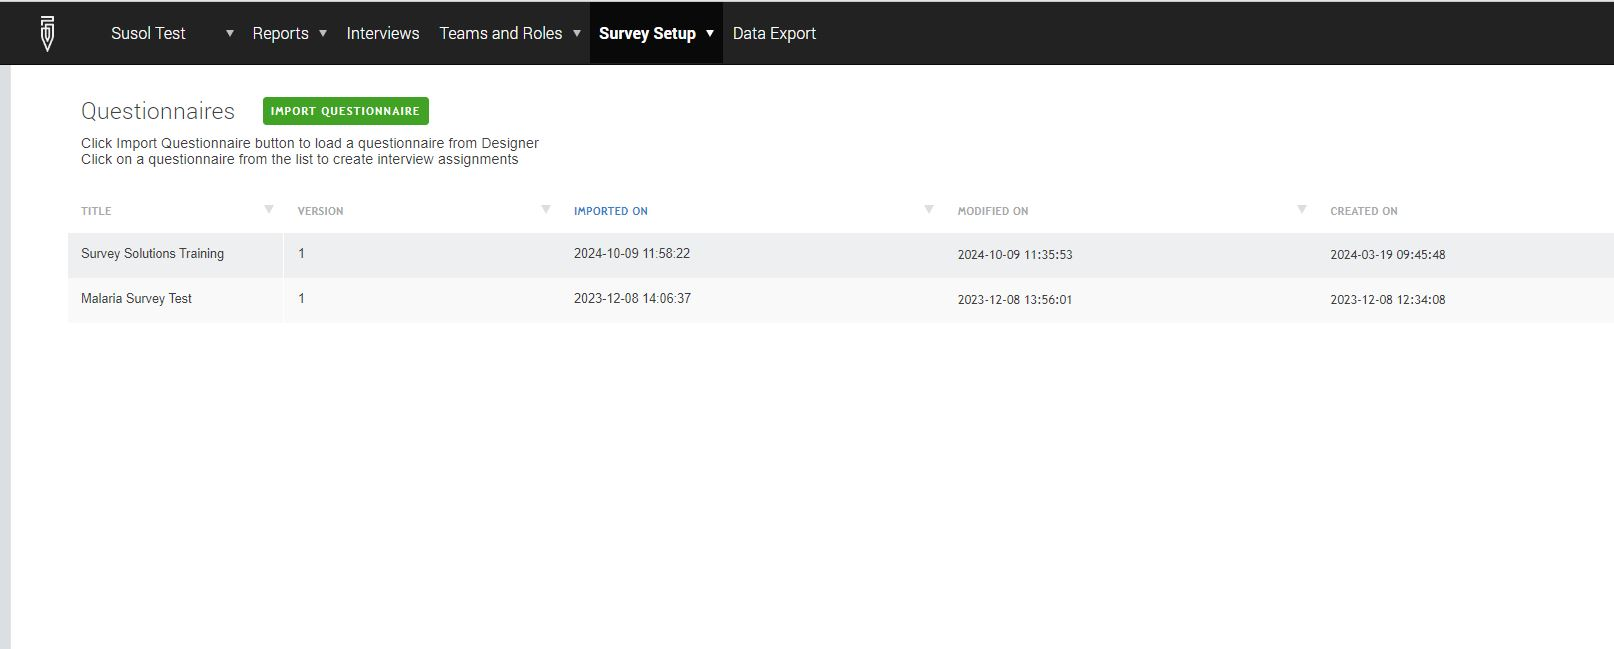
\includegraphics{images/login_susol.JPG}

  }

  \caption{Log in into the Survey Solution and pick the right workspace}

  \end{figure}%
\item
  \begin{figure}[H]

  {\centering 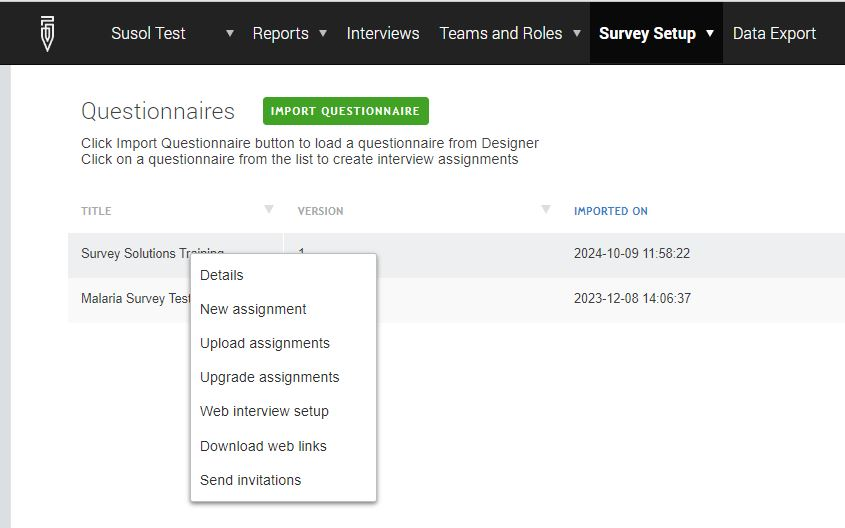
\includegraphics{images/click_quiz_details.JPG}

  }

  \caption{Click on desired questionnaire then select details}

  \end{figure}%
\item
  \begin{figure}[H]

  {\centering 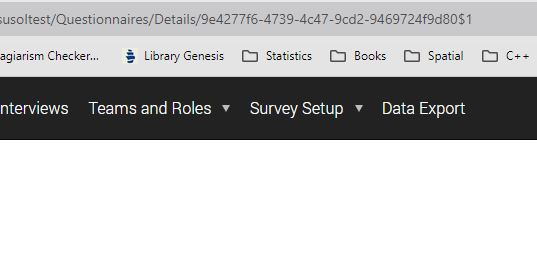
\includegraphics{images/quizid.JPG}

  }

  \caption{Locate the questionnaire at the address bar}

  \end{figure}%
\end{enumerate}

Between the \textbf{\emph{Details/}} and \textbf{\emph{\$}} sign is the
id.

\section{Download Script}\label{download-script}

The complete script to download data is given below:

\begin{Shaded}
\begin{Highlighting}[]
\CommentTok{\# Purpose: Download the trial dataset from the Survey Solutions server}
\CommentTok{\# Author: Moses Otieno}
\CommentTok{\# Date Created: 14 Oct 2024}
\CommentTok{\# Date Modified: 14 Oct 2024}

\CommentTok{\# {-}{-}{-}{-}{-} Modules required}

\ImportTok{import}\NormalTok{ requests}
\ImportTok{from}\NormalTok{ ssaw }\ImportTok{import}\NormalTok{ Client, ExportApi, QuestionnairesApi}
\ImportTok{from}\NormalTok{ ssaw }\ImportTok{import}\NormalTok{ models}
\ImportTok{from}\NormalTok{ time }\ImportTok{import}\NormalTok{ sleep}
\ImportTok{import}\NormalTok{ configparser}


\CommentTok{\# {-}{-}{-}{-} Read and get config values }

\NormalTok{config }\OperatorTok{=}\NormalTok{ configparser.ConfigParser()}
\NormalTok{config.read(}\StringTok{\textquotesingle{}config.ini\textquotesingle{}}\NormalTok{)}

\NormalTok{urls }\OperatorTok{=}\NormalTok{ [config[}\StringTok{\textquotesingle{}susol\textquotesingle{}}\NormalTok{][}\StringTok{\textquotesingle{}url\textquotesingle{}}\NormalTok{]]}

\NormalTok{survey\_test\_id }\OperatorTok{=}\NormalTok{ config[}\StringTok{\textquotesingle{}susol\textquotesingle{}}\NormalTok{][}\StringTok{\textquotesingle{}survey\_test\_id\textquotesingle{}}\NormalTok{]}
\NormalTok{mal\_id }\OperatorTok{=}\NormalTok{ config[}\StringTok{\textquotesingle{}susol\textquotesingle{}}\NormalTok{][}\StringTok{\textquotesingle{}mal\_id\textquotesingle{}}\NormalTok{]}

\CommentTok{\# {-}{-}{-}{-} Specify the questionnaires to download data from }

\NormalTok{questionnaires }\OperatorTok{=}\NormalTok{ \{}
    \StringTok{"survey\_test"}\NormalTok{: survey\_test\_id,}
    \StringTok{"malaria"}\NormalTok{: mal\_id}
\NormalTok{\}}


\CommentTok{\# {-}{-}{-}{-}{-} Define functions}

\KeywordTok{def}\NormalTok{ connect\_to\_internet(url}\OperatorTok{=}\StringTok{\textquotesingle{}http://www.google.com/\textquotesingle{}}\NormalTok{, timeout}\OperatorTok{=}\DecValTok{5}\NormalTok{):}
    \CommentTok{"""Check internet connectivity by pinging the given URL."""}
    \ControlFlowTok{try}\NormalTok{:}
\NormalTok{        \_ }\OperatorTok{=}\NormalTok{ requests.head(url, timeout}\OperatorTok{=}\NormalTok{timeout)}
        \ControlFlowTok{return} \VariableTok{True}
    \ControlFlowTok{except}\NormalTok{ requests.}\PreprocessorTok{ConnectionError}\NormalTok{:}
        \ControlFlowTok{return} \VariableTok{False}


\KeywordTok{def}\NormalTok{ connect\_to\_server():}
    \CommentTok{"""Attempt to connect to the Survey Solutions server via available URLs."""}
    \ControlFlowTok{for}\NormalTok{ url }\KeywordTok{in}\NormalTok{ urls:}
        \ControlFlowTok{if}\NormalTok{ connect\_to\_internet(url):}
            \BuiltInTok{print}\NormalTok{(}\SpecialStringTok{f\textquotesingle{}Connected to server: }\SpecialCharTok{\{}\NormalTok{url}\SpecialCharTok{\}}\SpecialStringTok{\textquotesingle{}}\NormalTok{)}
            \ControlFlowTok{return}\NormalTok{ url}
    \BuiltInTok{print}\NormalTok{(}\StringTok{"No connection to any server."}\NormalTok{)}
    \ControlFlowTok{return} \VariableTok{None}


\KeywordTok{def}\NormalTok{ get\_questionnaire\_versions(client, questionnaire\_id):}
    \CommentTok{"""Retrieve all versions of a questionnaire."""}
    \ControlFlowTok{return}\NormalTok{ [(q.}\BuiltInTok{id}\NormalTok{, q.version) }\ControlFlowTok{for}\NormalTok{ q }\KeywordTok{in}\NormalTok{ QuestionnairesApi(client).get\_list(questionnaire\_id}\OperatorTok{=}\NormalTok{questionnaire\_id)]}


\KeywordTok{def}\NormalTok{ download\_questionnaire\_data(client, qid, version, export\_path}\OperatorTok{=}\StringTok{\textquotesingle{}data\textquotesingle{}}\NormalTok{):}
    \CommentTok{"""Export and download questionnaire data in STATA format."""}
    \ControlFlowTok{try}\NormalTok{:}
\NormalTok{        export\_object }\OperatorTok{=}\NormalTok{ models.ExportJob(qid, export\_type}\OperatorTok{=}\StringTok{\textquotesingle{}STATA\textquotesingle{}}\NormalTok{)}
\NormalTok{        ExportApi(client).start(export\_object, wait}\OperatorTok{=}\VariableTok{True}\NormalTok{)}
\NormalTok{        ExportApi(client, workspace}\OperatorTok{=}\StringTok{"susoltest"}\NormalTok{).get(questionnaire\_identity}\OperatorTok{=}\NormalTok{qid, export\_type}\OperatorTok{=}\StringTok{\textquotesingle{}STATA\textquotesingle{}}\NormalTok{, show\_progress}\OperatorTok{=}\VariableTok{True}\NormalTok{, generate}\OperatorTok{=}\VariableTok{True}\NormalTok{, export\_path}\OperatorTok{=}\NormalTok{export\_path)}
        \BuiltInTok{print}\NormalTok{(}\SpecialStringTok{f\textquotesingle{}Successfully downloaded version: }\SpecialCharTok{\{}\NormalTok{version}\SpecialCharTok{\}}\SpecialStringTok{\textquotesingle{}}\NormalTok{)}
    \ControlFlowTok{except} \PreprocessorTok{Exception} \ImportTok{as}\NormalTok{ e:}
        \BuiltInTok{print}\NormalTok{(}\SpecialStringTok{f\textquotesingle{}Failed to download version: }\SpecialCharTok{\{}\NormalTok{version}\SpecialCharTok{\}}\SpecialStringTok{. Error: }\SpecialCharTok{\{}\NormalTok{e}\SpecialCharTok{\}}\SpecialStringTok{\textquotesingle{}}\NormalTok{)}


\KeywordTok{def}\NormalTok{ download\_all\_versions(client, qnrids, qnrversions):}
    \CommentTok{"""Loop through all versions of a questionnaire and download data."""}
    \ControlFlowTok{for}\NormalTok{ qnrid, version }\KeywordTok{in} \BuiltInTok{zip}\NormalTok{(qnrids, qnrversions):}
\NormalTok{        download\_questionnaire\_data(client, qnrid, version)}


\CommentTok{\# {-}{-}{-}{-}{-} Main execution logic}
\KeywordTok{def}\NormalTok{ main():}
    \CommentTok{\# Connect to the server and check internet connectivity}
\NormalTok{    server\_url }\OperatorTok{=} \VariableTok{None}
    \ControlFlowTok{for}\NormalTok{ attempt }\KeywordTok{in} \BuiltInTok{range}\NormalTok{(}\DecValTok{1}\NormalTok{, }\DecValTok{2}\NormalTok{):}
        \BuiltInTok{print}\NormalTok{(}\SpecialStringTok{f\textquotesingle{}Attempt }\SpecialCharTok{\{}\NormalTok{attempt}\SpecialCharTok{\}}\SpecialStringTok{ to connect...\textquotesingle{}}\NormalTok{)}
\NormalTok{        server\_url }\OperatorTok{=}\NormalTok{ connect\_to\_server()}
        \ControlFlowTok{if}\NormalTok{ server\_url:}
            \ControlFlowTok{break}
\NormalTok{        sleep(}\DecValTok{5}\NormalTok{)}
    \ControlFlowTok{if} \KeywordTok{not}\NormalTok{ server\_url:}
        \BuiltInTok{print}\NormalTok{(}\StringTok{"Failed to connect after 10 attempts."}\NormalTok{)}
        \ControlFlowTok{return}

    

    \CommentTok{\# Retrieve necessary configuration details}
\NormalTok{    api\_user }\OperatorTok{=}\NormalTok{ config[}\StringTok{\textquotesingle{}susol\textquotesingle{}}\NormalTok{][}\StringTok{\textquotesingle{}api\_user\textquotesingle{}}\NormalTok{]}
\NormalTok{    passwd }\OperatorTok{=}\NormalTok{ config[}\StringTok{\textquotesingle{}susol\textquotesingle{}}\NormalTok{][}\StringTok{\textquotesingle{}api\_password\textquotesingle{}}\NormalTok{]}
\NormalTok{    wkspace }\OperatorTok{=}\NormalTok{ config[}\StringTok{\textquotesingle{}susol\textquotesingle{}}\NormalTok{][}\StringTok{\textquotesingle{}workspace\textquotesingle{}}\NormalTok{]}
\NormalTok{    quizid }\OperatorTok{=}\NormalTok{ config[}\StringTok{\textquotesingle{}susol\textquotesingle{}}\NormalTok{][}\StringTok{\textquotesingle{}quiz\_id\textquotesingle{}}\NormalTok{]}

   \CommentTok{\# Initialize the Survey Solutions client}
   
\NormalTok{    client }\OperatorTok{=}\NormalTok{ Client(url}\OperatorTok{=}\NormalTok{server\_url, api\_user}\OperatorTok{=}\NormalTok{api\_user, api\_password}\OperatorTok{=}\NormalTok{passwd, workspace}\OperatorTok{=}\NormalTok{wkspace)}

    \CommentTok{\# Process each questionnaire}
    
    \ControlFlowTok{for}\NormalTok{ quizname, quizid }\KeywordTok{in}\NormalTok{ questionnaires.items():}
\NormalTok{        qnr\_data }\OperatorTok{=}\NormalTok{ get\_questionnaire\_versions(client, quizid)}
        \ControlFlowTok{if}\NormalTok{ qnr\_data:}
\NormalTok{            qnrids, qnrversions }\OperatorTok{=} \BuiltInTok{zip}\NormalTok{(}\OperatorTok{*}\NormalTok{qnr\_data)}
            \BuiltInTok{print}\NormalTok{(}\SpecialStringTok{f\textquotesingle{}The highest version of }\SpecialCharTok{\{}\NormalTok{quizname}\SpecialCharTok{\}}\SpecialStringTok{ is }\SpecialCharTok{\{}\BuiltInTok{max}\NormalTok{(qnrversions)}\SpecialCharTok{\}}\SpecialStringTok{. Downloading versions from }\SpecialCharTok{\{}\BuiltInTok{min}\NormalTok{(qnrversions)}\SpecialCharTok{\}}\SpecialStringTok{ to }\SpecialCharTok{\{}\BuiltInTok{max}\NormalTok{(qnrversions)}\SpecialCharTok{\}}\SpecialStringTok{.\textquotesingle{}}\NormalTok{)}
\NormalTok{            download\_all\_versions(client, qnrids, qnrversions)}
        \ControlFlowTok{else}\NormalTok{:}
            \BuiltInTok{print}\NormalTok{(}\SpecialStringTok{f\textquotesingle{}No versions found for }\SpecialCharTok{\{}\NormalTok{quizname}\SpecialCharTok{\}}\SpecialStringTok{.\textquotesingle{}}\NormalTok{)}

\ControlFlowTok{if} \VariableTok{\_\_name\_\_} \OperatorTok{==} \StringTok{"\_\_main\_\_"}\NormalTok{:}
\NormalTok{    main()}
\end{Highlighting}
\end{Shaded}

\subsection{Customizing Download
Script}\label{customizing-download-script}

I\textquotesingle ve done my best to make things easy for you. However,
you need to provide specific details in the script to download your
data:

\begin{enumerate}
\def\labelenumi{\arabic{enumi}.}
\item
  \textbf{config.ini}: Create a \texttt{config.ini} file with a section
  called \textbf{susol}. Include the required details:
  \texttt{api\ user}, \texttt{api\ password}, \texttt{url}, and
  \texttt{workspace}.
\item
  \textbf{Questionnaire}: Identify the IDs of the questionnaires you
  want to download and add them to the config file.
\item
  \textbf{export\_path}: Specify the download directory for the data.
  The script assumes there\textquotesingle s a \textbf{data} directory
  in the same path; if not, create one or specify your desired
  directory.
\end{enumerate}

Once you have this information, you\textquotesingle ll be able to
download your data.

\subsection{Error Handling and
Debugging}\label{error-handling-and-debugging}

\begin{itemize}
\item
  If the script fails to connect, check your internet connection and the
  details in \texttt{config.ini}.
\item
  If you receive an ``Invalid Questionnaire ID'' error, verify that the
  IDs in the \texttt{questionnaires} dictionary are correct.
\item
  Monitor the output messages for any errors during the download
  process.
\end{itemize}

\subsection{Convention: Assigning One Workspace to One
Directory}\label{convention-assigning-one-workspace-to-one-directory}

In many data management and programming workflows, particularly when
dealing with multiple datasets, scripts, and configurations,
establishing a clear and consistent directory structure is essential for
maintaining organization and efficiency. I strongly advocate for the
convention of assigning one workspace to one directory. A workspace can
contain multiple questionnaires, so this script assumes that you will
work with each workspace separately.

\section{Summary}\label{summary}

Below is a summary of the steps you need to undertake in order to
download data from Survey Solutions server to your machine.

\begin{itemize}
\tightlist
\item
  \textbf{Create API User}: Ensure you have an API user created.
\item
  \textbf{Gather Information}: Collect the following:

  \begin{itemize}
  \item
    URL
  \item
    API username
  \item
    API password
  \item
    Workspace
  \item
    Questionnaire ID
  \end{itemize}
\item
  \textbf{Install \texttt{ssaw} Module}: Use Python to install the
  \texttt{ssaw} module.
\item
  \textbf{Create .ini Config File}: Store all necessary information for
  the Survey Solutions Server.
\item
  \textbf{Run the Script}: Execute the script to download the data!
\end{itemize}

\bookmarksetup{startatroot}

\chapter{Data Import}\label{data-import}

\section{Introduction}\label{introduction-2}

After downloading the data, the next step is to import it into your
programming environment for analysis. This section on data import is
essential because Survey Solutions stores the downloaded data in a
specific format. In our download script, we specified
\texttt{export\_type=\textquotesingle{}STATA\textquotesingle{}}, which I
prefer because STATA files include both variable labels and value
labels, eliminating the need to redefine them. Additionally, note that
the downloaded data is in a zipped format. If you have two versions of a
questionnaire, you'll receive two separate zipped files. There are two
ways you can import this data into R:

\begin{enumerate}
\def\labelenumi{\arabic{enumi}.}
\item
  \textbf{Manual Import}: undefined
\item
  \textbf{Automated Import}: Use a script to handle all the importing
  procedures, streamlining the process.
\end{enumerate}

\bookmarksetup{startatroot}

\chapter*{References}\label{references}
\addcontentsline{toc}{chapter}{References}

\markboth{References}{References}

\phantomsection\label{refs}
\begin{CSLReferences}{0}{1}
\end{CSLReferences}




\end{document}
